\documentclass{standalone}
\usepackage{xcolor}
\definecolor{colorbrewer1}{RGB}{228,26,28}
\definecolor{colorbrewer2}{RGB}{55,126,184}
\definecolor{colorbrewer3}{RGB}{77,175,74}
\definecolor{colorbrewer4}{RGB}{152,78,163}
\definecolor{colorbrewer5}{RGB}{255,127,0}
\definecolor{colorbrewer6}{RGB}{255,255,51}
\definecolor{colorbrewer7}{RGB}{166,86,40}
\definecolor{colorbrewer8}{RGB}{247,129,191}
\definecolor{colorbrewer9}{RGB}{153,153,153}
\usepackage[scaled]{helvet}
\usepackage{tikz}
\graphicspath{{../}{../../Stutz2019CVPR/}{/BS/dstutz/work/robustness-cvpr/Stutz2019CVPR/}{/home/dstutz/robustness-cvpr/Stutz2019CVPR/}}
\usepackage{tikz-3dplot}
\usetikzlibrary{fadings}
\usepackage[active,tightpage]{preview}
\PreviewEnvironment{tikzpicture}
%\setlength\PreviewBorder{2mm}
\renewcommand{\rmdefault}{phv}
\renewcommand{\sfdefault}{phv}
\renewcommand{\ttdefault}{pcr}
\begin{document}

    %set the plot display orientation
    %synatax: \tdplotsetdisplay{\theta_d}{\phi_d}
    \tdplotsetmaincoords{72.5}{20}
    %define xy plane
    \tikzset{yxplane/.style={canvas is yx plane at z=#1}}
    
    \begin{tikzpicture}[scale=5,tdplot_main_coords]    
        %\begin{scope}[shift={(0.075,0.05,0.35)}]
        %    \draw[->,black] (-0.5,-0.5,0.5) -- (-0.25,-0.5,0.5) node[anchor=west,xshift=-0.05cm,white]{\footnotesize $x$};
        %    \draw[->,black] (-0.5,-0.5,0.5) -- (-0.5,-0.25,0.5) node[anchor=south west,xshift=-0.075cm,yshift=-0.075cm,white]{\footnotesize $y$};
        %    \draw[->,black] (-0.5,-0.5,0.5) -- (-0.5,-0.5,0.75) node[anchor=south,yshift=-0.05cm,white]{\footnotesize $z$};
        %\end{scope}
        
        \begin{scope}[yxplane=1]
            \draw[draw=black] (0, 0) circle[radius=0.5cm] node{};
            
            \coordinate (o) at (0.1,0){};
            \draw[thick,draw=black,fill=black] (o) circle[radius=0.15mm] node{};
            \node at ($(o) + (-0.075,0.05)$){$x$};
            
            \draw[thick,draw=black,fill=black] (0.1, -0.4) circle[radius=0.15mm] node (3){};
            \node at ($(3) + (-0.075,-0.025)$){$x_3$};
            
            \draw[thick,draw=black,fill=black] (-0.27, 0.23) circle[radius=0.15mm] node (2){};
            \node at ($(2) + (-0.075,-0.025)$){$x_2$};
            
            \draw[thick,draw=black,fill=black] (0.1, 0.15) circle[radius=0.15mm] node (1){};
            \node at ($(1) + (-0.075,-0.025)$){$x_1$};
            
            \draw[thick,draw=black,fill=black] (-0.25,-0.25) circle[radius=0.15mm] node (4){};
            \node at ($(4) + (-0.075,-0.025)$){$x_4$};
        \end{scope}
        
        \coordinate (off) at ($(o) + (-0.2,0.1,0.325)$);
        \node[anchor=north west,yshift=0.1cm] at (off){$\tilde{x}$};
        \draw[thick,draw=colorbrewer1,fill=colorbrewer1] (off) circle[radius=0.1mm];
        \draw[->] (o) -- (off);
        \draw[-,dashed] (o) -- ($(o) + (-0.2,0.1,0)$);
        
        \draw[-,dashed] ($(o) + (-0.2,0.1,0)$) -- (off);
        \node[anchor=east,yshift=0.6cm] at ($(o) + (-0.125,-0.1,0.05)$){$\|\tilde{x} - \pi(\tilde{x})\|_2$};
        
        \node[anchor=north east,yshift=0.1cm,xshift=0.05] at (off){
\includegraphics[width=0.75cm]{gfx/introduction/off_manifold/152_0_attack_9.png}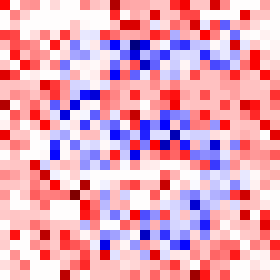
\includegraphics[width=0.75cm]{{gfx/introduction/off_manifold/152_0_perturbation_0.3}.png}};
        \node[anchor=south,yshift=-0.1cm,xshift=-0.1cm] at (off){\begin{tabular}{@{}l@{}} regular\\[-1px]adversarial example\end{tabular}};
        
        \node[anchor=north east,xshift=0.05cm,yshift=0.05cm] at (o){
\includegraphics[width=0.75cm]{gfx/introduction/off_manifold/152_0_image_5}};
        
        \node at ($(o) + (0.325,-1)$){\bfseries \begin{tabular}{c}Approximate Manifold using\\Nearest Neighbors\end{tabular}};
        
    \end{tikzpicture}
\end{document}